The comparison of different architectures in a fair manner is not trivial to do.
Because it is possible that the performance of an architecture is highly dependent on the used hyperparameters, for a fair comparison it would be necessary to optimize the hyperparameters for every architecture and only compare the top scoring results.
As performing training runs for this thesis takes durations ranging from \SI[]{30}[]{\minute} to \SI[]{12}[]{\hour}, it is not feasible to run the powerset of hyperparameter combinations and choose only the best.
Even with the resources provided by Augsburg University to calculate a higher number of runs than were ever possible on only my local machines, investing months into these calculations is neither possible, nor sensible.

Therefore an informed pre-selection of likely interesting runs had to be chosen beforehand.
Helpful in this manner were the previous experiences by other researchers. 
The metaformer's hyperparameters \emph{image size}, \emph{number of heads}, \emph{patch size}, \emph{embed dimension}, \emph{depth} and \emph{mlp ratio} have been chosen as the same values, the \emph{DINO tiny} model was implemented in \cite{dinoGithub}. As the transformer in the DINO paper \cite{dinoPaper} was a structural template for this metaformer, selecting the smallest model from their lineup made it possible to perform as many comparisons as possible with limited resources.

In order to understand what is measured a full overview of the recorded parameters is presented in \autoref{fig:comparison-recorded-values}.

\begin{figure}[htbp]
    \centering
    \makebox[\textwidth][c]{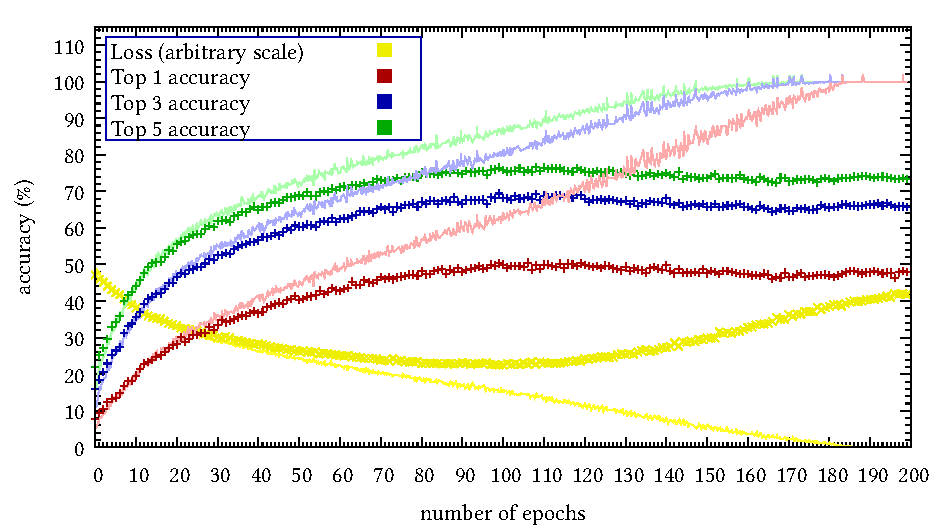
\includegraphics[width=1.1\textwidth]{./experiments/image-classification/training-settings/metrics/metrics.pdf}}
    \caption{Graphic depiction of all recorded metrics for the image classification task.
    The data is from a \emph{CF} metaformer and has been selected because it clearly shows the expected behavior of convergence.
    The \emph{accuracy} (\autoref{sec:theory-imageclassification}) and \emph{loss} (\autoref{sec:theory-neuralnetworktraining}) are depicted. 
    The results from \emph{testing} the model on the validation set are depicted as individual data points and colored dark. 
    The data collected during the \emph{training} calculations are colored in the corresponding color, but shaded more brightly. The training data is plotted as a smoothed line, to allow for a more pleasant viewing experience.
    The loss data is scaled arbitrarily to fit into the graph, as the absolute values are not relevant. }
    \label{fig:comparison-recorded-values}
\end{figure}

All the runs share a few key similarities. Because of that that full data for one run is only shown once. 
Later figures will leave out most of the metrics, because they are almost completely redundant.

The model training always follows the same default structure: The accuracy starts low and the loss starts at a high value.
This is expected as in the beginning the model only guesses randomly. 
Therefore a top-1-accuracy should start at around \SI[]{1}[]{\percent} for a classification task of 100 classes.
It can be lower or higher depending on random chance, but in general it holds for very early values. 
As the results improve very rapidly in the first few epochs, this can not be seen in the charts for most runs.
Also it should be noted, that the first recorded \emph{test} data point is calculated \emph{after} the first epoch. 
The model therefore is already advanced and no longer random. 
This explains, why the curves start higher than expected.

A shared trend for all datasets is, that the top-3-accuracy lies above the top-1-accuracy and the top-5-accuracy above both. 
This is necessary, because if a model classifies the correct answer among the best three highest rated answers, it automatically has also classified it among the top five. 
Because of that only the performance for the top class predictions will be shown, as the other metrics provide not much  additional insight into the comparison between architectures.

It can also be observed, that the \emph{test} accuracy rises at first, then plateaus and finally falls off.
The \emph{training} accuracy however constantly rises and can even hit \SI[]{100}[]{\percent}.
This can be explained by overfitting (\autoref{sec:theory-neuralnetworktraining}).
As explained, the amount of training data is limited. 
Therefore the model is presented with the same image many times. 
As it is allowed to adjust its weights based on the training data, it is possible for it to \glqq remember\grqq{} all solutions.
As can be clearly seen by the descending test performance after a specific point, doing so is not helpful for classifying unseen images.
Overfitting can be counteracted by setting so called \emph{dropout} connections/weights.
By randomly setting weights to zero, the model is always restricted to a subset of its weights and therefore has to develop a more robust internal representation. This reduces/delays the overfitting behavior.

The goal however is to detect differences in the architectural design. 
Thus it is important to be able to differentiate whether a poolformer is inherently more robust to overfitting than a conformer or the other way around. Because of that the dropout always is set to zero.

Subsequently, all models were trained to the point of overfitting. 
If statements about the accuracy of a model are made, the highest value of the \emph{test accuracy} is presented.
For \autoref{fig:comparison-recorded-values} this is at epoch 106.
It can be noted, that this is also the point, at which the train loss starts to rise again.
As explained previously, the loss is a measure of model's performance. 
The smaller the loss, the better the representation. 
If the test loss is rising and the train loss is still falling, this is a clear indication for the model being in the process of overfitting. 
This can be summarized to the rule, that all models were trained to the point, where either the test accuracy was noticeably dropping or the test loss was noticeably rising.
If accuracies are plotted, that have no clearly visible drop-off at the end, this is because the overfitting could be recognized in trend of the loss. 
Calculations then often were aborted to save resources.

\begin{figure}[htbp]
    \centering
    \makebox[\textwidth][c]{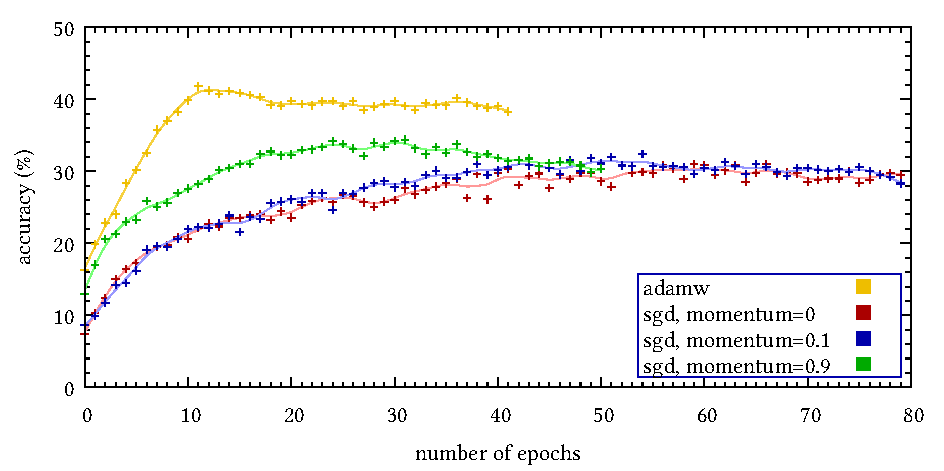
\includegraphics[width=1.1\textwidth]{./experiments/image-classification/training-settings/optimizer/optimizer.pdf}}
    \caption{Comparison of the top-1-accuracy for training a modified DINO tiny transformer.
    Different optimizer algorithms are used for the backpropagation.
    The training accuracy is pictured, the lighter colored lines are interpolations of the data with cubic splines. 
    This is supposed to make the differentiation of the red and blue curve easier.
    }
    \label{fig:optimizer}
\end{figure}

\autoref{fig:optimizer} shows a subset of the experiments performed to chose an appropriate \emph{optimizer} and learning rate.
It can be easily seen, that the choice of optimization algorithm influences the speed of convergence, as well as the maximum performance of the networks.
The \emph{adamw} \cite{adamwOptimizer} optimizer performed best in both of these metrics.
The established \emph{stochastic gradient descent} update algorithm scored a between \SIrange[]{10}{15}{\percent} worse test accuracy, as well as a two to four times slower rate of convergence in relation to the number of epochs.

Increasing the momentum value comes with no additional costs or drawbacks, however it leads to overall better performing models, that converge faster \cite{momentum}.
Because of that \SI{0.9}{} was chosen as the momentum value for the sgd in all subsequent runs.

In literature, multiple comparisons between the different optimization mechanisms have been performed \cite{sgdOrAdamw}.
Though the adamw optimizer performed better, the update procedure is also more expensive, in particular requiring more memory.
Because of that, the batch size could not be set to 128 (like for the sgd optimizer), but had to be reduced to 64, as the available GPU memory was quite limited at the start of the experiments.
At the same time, the sgd algorithm produced more consistent trends with less abrupt changes.
In order to again choose reliable comparability above maximum performance, only the sgd optimizer is used in subsequent image recognition experiments. 

All of the optimizers use a constant \emph{learning rate} of \SI[]{0.001}{}{}.